\section{Environtment Setup For Python}
Bahasa pemrograman python tersedia diberbagai platform, termasuk juga terdapat pada 
linux dan max os x. Untuk mengecek apakah python sudah terinstall atau belum, pertama 
tama bukalah command prompt atau terminal komputer dan ketikan python. Akan muncul info 
atau status mengenai apakah python sudah terinstall dan berapa versinya atau belum terinstall sama sekali.
  \begin{figure}[ht]
	\centerline{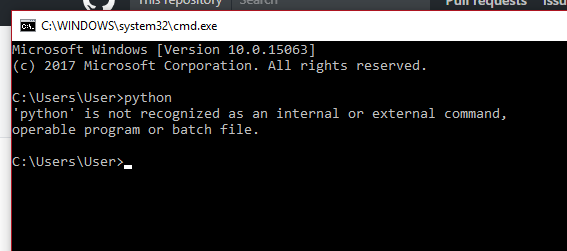
\includegraphics[width=1\textwidth]{Plagiarisme/cmd.PNG}}
	\caption{Contoh skirpt pada command prompt.}
	\label{cmd}
	\end{figure}
Pada gambar \ref{cmd} memberitahukan bahwa pada komputer yang saya pakai sekarang ini belum ada atau belum terinstall python.
Ketika python belum terinstall maka sistem akan mendeteksi bahwa comand yang diberikan tidak cocok dengan yang ada disistem. 
Akan tetapi kalau sudah terinstall maka akan memunculkan nama python begitu pula versi python yang di install.
Python menyediakan dukungan yang kuat untuk integrasi dengan bahasa pemrograman lain dan alat-alat bantu lainnya. 
Python hadir dengan pustakapustaka standar yang dapat diperluas serta dapat dipelajari hanya dalam beberapa hari.
Sudah banyak programmer Python yang menyatakan bahwa mereka mendapatkan produktivitas yang lebih tinggi. 
Mereka juga merasakan bahwa Python meningkatkan kualitas 
Distribusi Python tersedia untuk berbagai macam platform.
Anda hanya perlu mendownload kode biner yang berlaku untuk platform Anda dan menginstal Python.
Jika kode biner untuk platform Anda tidak tersedia, Anda memerlukan kompiler C untuk mengkompilasi kode sumber secara manual. 
Kompilasi kode sumber menawarkan fleksibilitas lebih dalam hal pilihan fitur yang Anda butuhkan dalam instalasi Anda.
Berikut adalah ikhtisar singkat tentang menginstal Python di berbagai platform

\subsection{installasi Python pada windows}
	\begin{enumerate}
	\item Unduh Python 2.7 di python.org.
	\item Jalankan file instalasi Python yang telah diunduh. Secara default Python akan terinstall di folder C:>Python27.
	\item Selanjutnya mengatur variable environment, buka Control Panel->System and Security->System.
	\item Klik Advanced system settings, Environment Variables.
	\item Pada System variables, pilih Path, klik Edit.
	\item Pada Variable value, tambahkan ;C:>Python27.
	\end{enumerate}
	
\subsubsection{Pengujian Python pada windows}
	\begin{enumerate}
	\item Cara pertama: ketik python untuk menjalankan Python Interpreter. 
	      Jika berhasil akan ditampilkan versi Python yang digunakan beserta interpreternya. 
	      Coba ketikkan print “hello world” untuk menampilkan teks hello world.
	\item Cara kedua: buat file hello.py, yang isinya print “hello world”, 
	      simpan di mana saja suka-suka kamu, misalnya di D:>python-code. Buka command prompt, Run -> cmd. 
	      Kemudian masuk ke folder D:>python-code, lalu ketik python hello.py untuk menjalankan file Python yang telah dibuat.

\subsection{Installasi Python pada Unix/Linux}
	Berikutini adalah simple steps untuk menginstall python pada Unix/Linux.
	\begin{enumerate}
	\item Buka web browser dan ketik alamat https://www.python.org/downloads/
	\item Ikuti link untuk mendownload source code yang bisa digunakan oleh Unix/Linux
	\item Download dan kemudian extrak file
	\item Edit modules/setup file jika mau customize beberapa pengaturan
	\item Jalankan perintah ./configure script
	\item Installasi 
	\end{enumerate}
Lokasi standar penginstallan python ada pada /usr/local/bin dan libraries nya berada 
/usr/local/lib/pythonXX dimana XX adalah versi python yang di install.

Pengujian
1.Cara pertama: ketik python untuk menjalankan Python Interpreter. Jika berhasil akan ditampilkan versi Python yang digunakan beserta interpreternya. Coba ketikkan print “hello world” untuk menampilkan teks hello world.

C:>python
Python 2.7.11 (v2.7.11:6d1b6a68f775, Dec  5 2015, 20:40:30) [MSC v.1500 64 bit (AMD64)] on win32
Type "help", "copyright", "credits" or "license" for more information.
>>> print "hello world"
hello world
>>>

Cara kedua: buat file hello.py, yang isinya print “hello world”, simpan di mana saja suka-suka kamu, misalnya di D:\python-code. Buka command prompt, Run -> cmd. Kemudian masuk ke folder D:\python-code, lalu ketik python hello.py untuk menjalankan file Python yang telah dibuat.

D:\python-code>python hello.py
hello world

